\documentclass[sigplan, anonymous, review]{acmart}

% Removes citation information below abstract
\settopmatter{printacmref=false, printcss=false, printfolios=true}
% removes footnote with conference information in first column
\renewcommand\footnotetextcopyrightpermission[1]{}
%% removes running headers
%% \pagestyle{plain}

\usepackage[active,float]{preview}
\PreviewEnvironment{tikzpicture}

\usepackage[T1]{fontenc}
\usepackage{algpseudocode}
\usepackage{amsmath}
\usepackage{booktabs} % For formal tables
\usepackage{enumitem}
\usepackage{hyperref}
\usepackage{listings}
\usepackage{multirow}
\usepackage{subcaption}
\usepackage{tikz}
\usepackage{varwidth}
\usepackage{xcolor}

\usetikzlibrary{calc, backgrounds, shadows, positioning}

%%
%% Define match case
%%
\algnewcommand\algorithmicmatch{\textbf{match}}
\algnewcommand\algorithmiccase{\textbf{case}}
\algnewcommand\Assert[1]{\State \algorithmicassert(#1)}
\algdef{SE}[MATCH]{Match}{EndMatch}[1]{\algorithmicmatch\ #1\ \algorithmicdo}{\algorithmicend\ \algorithmicmatch}%
\algdef{SE}[CASE]{Case}{EndCase}[1]{#1 $\Rightarrow$}{\algorithmicend\ \algorithmiccase}%
\algtext*{EndMatch}%
\algtext*{EndCase}%

\hypersetup{
  colorlinks=true,
  linkcolor=ACMRed,
  urlcolor=ACMBlue,
  citecolor=ACMRed,
}

\lstset{
  showspaces=false,
  showtabs=false,
  breaklines=true,
  showstringspaces=false,
  breakatwhitespace=true,
  escapeinside={(*@}{@*)},
  basicstyle=\scriptsize\ttfamily,
  columns=fullflexible,
  morekeywords={maybe_downsample, maybe_skip}
}

\captionsetup[figure]{belowskip=-8pt,aboveskip=7pt}
\captionsetup[table]{belowskip=5pt,aboveskip=7pt}

%% Copyright
\setcopyright{none}
% \setcopyright{acmcopyright}
% \setcopyright{acmlicensed}
% \setcopyright{rightsretained}
% \setcopyright{usgov}
% \setcopyright{usgovmixed}
% \setcopyright{cagov}
% \setcopyright{cagovmixed}

%% Below is commented out for submission
% % DOI
% \acmDOI{10.475/123_4}
% % ISBN
% \acmISBN{123-4567-24-567/08/06}

%% Conference
\acmConference[SOSP'17]{}{October 29--31, 2017}{Shanghai, China}
\acmYear{2017}
\copyrightyear{2017}
% \acmPrice{15.00}
% \acmBadgeL[http://ctuning.org/ae/ppopp2016.html]{ae-logo}

\begin{document}
\title{Resilient Wide-area Streaming Analytics \\
  with Automatic Profiling and Runtime Adaptation}

% The default list of authors is too long for headers}
\renewcommand{\shortauthors}{B. Zhang et al.}

\newcommand{\sysname}{AdaptiveStream}
\newcommand{\para}[1]{\medskip\noindent\textbf{#1}}
\newcommand{\paraf}[1]{\smallskip\noindent\textbf{#1}}
\newcommand{\todo}[1]{{\color{ACMRed}\bf{TODO: #1}\normalfont}}.

%%% Local Variables:
%%% mode: latex
%%% TeX-master: "sosp17"
%%% End:


\begin{abstract}
  In the wide area, the emerging class of streaming analytics faces the
  challenge of scarce and variable network bandwidth. Applications without
  adaptation suffer from increased latency or degraded accuracy. Existing
  approaches that adapt to network changes are often application-specific or
  require extensive developers' effort.

  This paper presents \sysname{}, a stream processing system that adapts the
  application execution with minimal developer efforts. To achieve this,
  \sysname{} employs three key ideas: (1) a novel set of APIs for structured
  adaptation; (2) a combination of offline and online profiling to construct a
  Pareto-optimal strategy; (3) a rate-based congestion control for runtime
  adaptation.

  We evaluate \sysname{} against three real-world applications including
  surveillance applications, augmented reality and distributed log analysis. At
  places where traditional approaches would lead to either significant
  application accuracy drop or long tail latency, our system gracefully
  maintains the balance between application accuracy and system performance.
\end{abstract}

% The code below should be generated by the tool at
% http://dl.acm.org/ccs.cfm
% Please copy and paste the code instead of the example below.
%
\begin{CCSXML}
<ccs2012>
  <concept>
    <concept_id>10010520.10010521.10010537</concept_id>
    <concept_desc>Computer systems organization~Distributed architectures</concept_desc>
    <concept_significance>300</concept_significance>
  </concept>
  <concept>
    <concept_id>10010520.10010570.10010574</concept_id>
    <concept_desc>Computer systems organization~Real-time system architecture</concept_desc>
    <concept_significance>300</concept_significance>
  </concept>
  <concept>
    <concept_id>10002951.10003227.10003251.10003255</concept_id>
    <concept_desc>Information systems~Multimedia streaming</concept_desc>
    <concept_significance>300</concept_significance>
  </concept>
  <concept>
    <concept_id>10002951.10003227.10010926</concept_id>
    <concept_desc>Information systems~Computing platforms</concept_desc>
    <concept_significance>300</concept_significance>
  </concept>
</ccs2012>
\end{CCSXML}

\ccsdesc[300]{Computer systems organization~Distributed architectures}
\ccsdesc[300]{Computer systems organization~Real-time system architecture}
\ccsdesc[300]{Information systems~Multimedia streaming}
\ccsdesc[300]{Information systems~Computing platforms}

%% Keywords are mostly obsolete, use CCS.
%% \keywords{adaptation, learning, stream processing}

%% Below is the code to create the teaser
% \begin{teaserfigure}
%   \includegraphics[width=\textwidth]{sampleteaser}
%   \caption{This is a teaser}
%   \label{fig:teaser}
% \end{teaserfigure}

\maketitle

\section{Introduction}

In this paper, we study streaming analytics in the wide area. Although recent
stream processing systems (such as Storm~\cite{toshniwal2014storm}, Spark
Streaming~\cite{zaharia2013discretized}) can handle large streams of data in a
single cluster, they are not designed to work in the wide area where the
bandwidth is not sufficient to backhaul all the data to a central location.

With the emerging class of Internet of Things (IoT) applications, such as video
surveillance and industrial monitoring, huge data volumes of data are generated
at the edge. In contrast, the Internet's available bandwidth is scarce and
varying, making it impossible to back-haul all the data. And the demand is
growing faster than the network capacity.

When the network resources become insufficient, applications have to choose
between data freshness and data fidelity. Applications based on TCP ensures a
reliable delivery of the data but the backlogged data will increase application
latency. Applications based on UDP could minimize latency by sending packets as
fast as possible, the uncontrolled packet loss along the network may devastate
the application. Either option is not ideal for many streaming anlaytics.

Previous work (JetStream~\cite{rabkin2014aggregation}) has explored the
direction of reducing application's demand with degradation, but it relies on
developers' manual policy, which lacks precision and faces scalability issue.
There are also application-specific optimizations; but they do not
generalize. For example, adaptive video streaming~\cite{yin2015control} is a
well-studied topic but many adaptations aim at human consumption, focusing on
Quality of Experience (QoE). This limits the adaptation space e.g. maintain
25FPS.

Making degradation practical and general across applications is challenging. The
goal is to maximizing application accuracy under the constrain of available
bandwidth with minimal developers' effort (with exhausting). It calls for the
right level of abstraction with a system-level approach.

In this work, we present \sysname{}, which aims to empower developers with an
easy-to-use framework for wide-area streaming analytics. We focus on the scarce
and variable bandwidth and solve it with three ideas: (1) a novel set of APIs
for structured adaptation; (2) a combination of offline and online profiling to
construct a Pareto-optimal strategy; (3) a rate-based congestion control for
runtime adaptation.

Our proposed API imposes a structure on the adaptation that each application can
perform; although the API is narrow, when combined with other operators, we find
the framework is expressive enough for many streaming analytics.

To liberate developers from specifying rules manually, our system employs a
data-driven empirical-analysis approach. The profiling is done both offline and
online. Offline profiling offers bootstrap information that makes online
profiling more efficient. Online profiling alleviates the problem of
\textit{model drift}.

The runtime adaptation automatically adjusts the applications' execution such
that the streaming demand matches the available bandwidth. We employs a
congestion-based congestion control scheme by measuring the bottleneck
bandwidth; in steady state, the system probes for more available bandwidth.

Using \sysname{}, we've built three applications: pedestrian detection,
augmented reality and distributed top-k. We use real-world data for these
applications to evaluate our systems.

The evaluation shows the generated profile for the three applications. Then for
each application, We show how they adapt the behavior at runtime. Under a
controlled experiment, even with only transient network capacity drop, our
system is able to maintain an end-to-end delay for 1 seconds in the wide-area
and accuracy level above 80\%. Application-agnostic protocols creates
significant backlogged data (TCP for about 100 seconds) or unusable accuracy
(UDP).

In summary, this paper makes the following contributions:

\begin{itemize}[leftmargin=16pt]
\item We study in depth of wide-area streaming applications in the case of
  network resource variation.
\item We propose a novel set of APIs to allow for structured adaptation: they
  require minimal developer efforts while being precise with automatic
  profiling.
\item We propose a new congestion control scheme that adapts the application
  data to available bandwidth, with a goal of minimizing the latency.
\item We implement a prototype system.
\item We build three real-world applications and evaluate their behavior
  under different scenarios.
\end{itemize}

%%% Local Variables:
%%% mode: latex
%%% TeX-master: "sosp17"
%%% End:

\begin{figure}
  \centering
  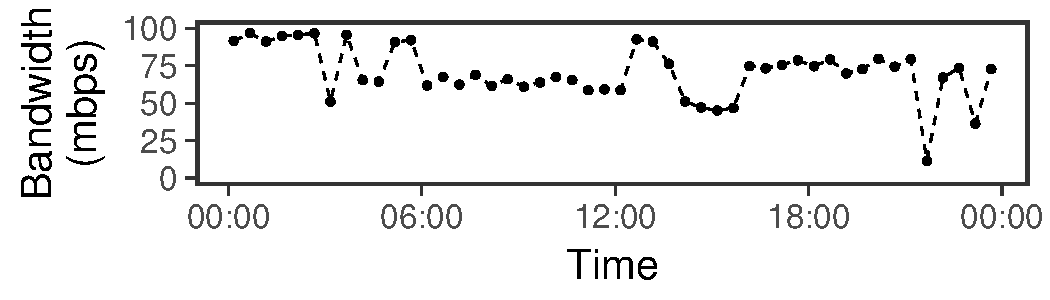
\includegraphics[width=.9\linewidth]{figures/aws-variation.pdf}
  \caption{Bandwidth variations throughout the day between Amazon EC2 sites
    (from Ireland to California).}
  \label{fig:bw}
\end{figure}

\begin{figure*}
  \centering
  \includegraphics[width=0.95\linewidth]{figures/motiv-app-specific.pdf}
  \caption{The measured bandwidth and application accuracy for two video analytics applications.
  (1) Different degradation strategies have different impacts on accuracy, e.g., degrading frame rate in (a) vs.\,degrading resolution in (b).
  (2) The same degradation strategy has different impacts on different applications, e.g., degrading frame rates works well for stationary camera (a), but not well for mobile camera (e). (c-g) shows example measurement frames.}
  \label{fig:app-specific}
\end{figure*}

\section{Motivation}
\label{sec:motivation}

In this section, we examine the gap between high application demands and limited
wide-area bandwidth. We then show that neither manual policies nor
application-specific optimizations solve the problem.

\subsection{Wide-area Streaming Applications}
\label{sec:wide-area-streaming}

\paraf{Video Surveillance.} We envisage a city-wide monitoring system that
aggregates camera feeds---from stationary ground cameras and moving aerial
vehicles---and analyzes video streams in real-time for surveillance, anomaly
detection or business intelligence~\cite{oh2011large}. Traditionally, video
analysis has relied on humans, but recent advances in computer vision and deep
learning have dramatically increased accuracy for automatic visual scene analysis,
such as pedestrian detection~\cite{dollar2012pedestrian}, vehicle
tracking~\cite{coifman1998real}, an facial recognition to locate people of
interest~\cite{parkhi2015deep, Lu:2015:SHF:2888116.2888245}. While some
surveillance networks use dedicated links, an increasing number of surveillance
systems, such as Dropcam~\cite{dropcam} and Vigil~\cite{zhang2015design}, use
the public Internet and wireless links to reduce the cost of deployment and
management.

% \para{High-frequency IoT Sensors:} Although environmental sensors used to be
% slow and not data-intensive~\cite{atzori2010internet}, increasingly,
% high-frequency, high-precision sensors are deployed. For example, uPMUs
% monitor the electrical grid with a network of 1000 devices; each produces 12
% streams of 120 Hz high-precision values accurate to 100 ns. This amounts to
% 1.4 million points per second~\cite{andersen2016btrdb}.

\para{Infrastructure Monitoring.} Large organizations today are managing
10--100s of data centers (DCs) and edge clusters
worldwide~\cite{calder2013mapping}. This geo-distributed infrastructure
continuously produces large volumes of data such as data access logs, server
monitoring logs, and performance counters~\cite{pu2015low,
  alspaugh2014analyzing, vulimiri2015global}. While most log analysis today runs
in batch mode on a daily basis, there is a trend towards analyzing logs in real
time for rapid optimization~\cite{rabkin2014aggregation}. For example, CDNs can
improve the overall efficiency by optimizing data placement if the access logs
can be processed in real time.

%% ~\cite{xu2009detecting} We generated the HDFS logs by setting up a Hadoop
%% cluster on 203 EC2 nodes and running sample Hadoop map-reduce jobs for 48
%% hours, generating and processing over 200 TB of random data. We collected
%% over 24 million lines of logs from HDFS.

% We consider the practical issues with deploying these applications in the
% wide-area. Our stand is that these applications face a bigger network
% challenge.  Data generated from the edge often fail to be delivered to the
% processing site because of the scarce and variable bandwidth capacity in the
% wide-area. Once they arrive, existing stream processing systems can easily
% manage a large cluster and perform data analytics at real-time.

\subsection{Wide-area Bandwidth Characteristics}
\label{sec:wide-area-bandwidth}

WAN bandwidth is insufficient and costly, as demonstrated by recent WAN-aware
systems~\cite{pu2015low, vulimiri2015global, vulimiri2015wananlytics,
  hsieh17gaia}. Using Amazon EC2 as a case study, the WAN bandwidth capacity is
15x smaller than their LAN bandwidth on average, and up to 60x smaller in the
worst case~\cite{hsieh17gaia}. In terms of pricing, as of April 2017, the
average WAN bandwidth cost is up to 38x of the cost of renting two
machines~\cite{amazon2017pricing, hsieh17gaia}.

In addition to the scarcity and cost, the large variability of WAN bandwidth
also affects streaming workloads. We conducted a day-long measurement using
iPerf~\cite{iperf3} to measure pair-wise bandwidth between four Amazon EC2
sites. The results show large variance in all pairs---\autoref{fig:bw} is one
such pair. There are occasions when available bandwidth is below 25\% of the
maximum bandwidth.

The back-haul links between EC2 sites are better---if not at least
representative---in comparison to general WAN links. Similar scarcity and
variations have been reported in wireless networks~\cite{biswas2015large},
broadband access networks~\cite{grover2013peeking, sundaresan2014bismark} and
cellular networks~\cite{nikravesh2014mobile}.

\subsection{The Case for a System Approach}
\label{sec:making-case-sys-approach}

To address the bandwidth limits, existing solutions include manual policies and
application-specific solutions. We discuss their drawbacks to make the case for
a system approach.

\para{Manual polices are sub-optimal.} While existing systems such as
JetStream~\cite{rabkin2014aggregation} and DASH~\cite{sodagar2011mpeg} allow
adaptation, they require developers to write manual policies. We illustrate the
problems with manual policies using an example~\cite{rabkin2014aggregation}:
\textit{if bandwidth is insufficient, switch to sending images at 75\% fidelity,
  then 50\% if there still isn't enough bandwidth. Beyond that point, reduce the
  frame rate, but keep the image fidelity.}

First, this policy is not accurate.
Developers write such rules based on heuristics and
don't back them up with measurements. Images with 75\% fidelity do not
necessarily lead to 75\% application accuracy. In terms of bandwidth, naively
one would think that reducing the frame rate by half will also half the data
rate. But if video encoding such as H.264~\cite{richardson2011h} is used, a reduction in frame rate increases the inter-frame difference, creating
larger P-frames. \hyperref[fig:app-specific]{Fig.~3e} shows that by reducing the
frame rate to one-third (from \(30~\text{FPS}\) to \(10~\text{FPS}\)), the bandwidth demand is still more than 50\%.

Second, it is not scalable to specify rules in this way. When the policy involves multiple dimensions
or developers desire a fine-grain control, the policy will end up with too many
rules.  Writing such rules manually is a tedious and error-prone process.

Lastly, this abstraction is too low-level. It forces developers to study and measure the
impact of individual operations, prohibiting its wide adoption in practice.

\para{Application-specific solutions don't generalize.} Because each application
has a different performance metric, relies on different features, and targets
different data distributions, a fine-tuned policy for one application will often work
poorly for others.

Analytical applications have their own goals, entailing different optimization metrics and
different algorithms.
%
%For instance, traditional video streaming focuses on end-users'
%experience~\cite{yin2015control, michalos2012dynamic, pantos2016http}. If we
%transfer their techniques to %machine-based video analytics, the %system maintains
%an unnecessarily-high frame rate.
%
In video analytics, for instance,
object detection algorithms depend on the edge
information~\cite{canny1986computational, lowe2004distinctive, viola2001rapid}
while object tracking~\cite{allen2004object} works best when the inter-frame
difference is small. The former is sensitive to resolution changes while the
latter frame rate changes.

Similar applications face different data distributions. Compare the stationary
camera detecting pedestrians with the mobile camera recognizing objects
(\autoref{fig:app-specific}). In the former case, when we take the pedestrians'
walking speed into consideration, a high frame rate is not necessary. But
high-resolution images are crucial as surveillance cameras are far from the
targets. In the latter case, mobile cameras move. Reducing the frame rate
introduces significant errors.

%%% Local Variables:
%%% mode: latex
%%% TeX-master: "awstream"
%%% End:

\section{\sysname{}}
\label{sec:system}

\sysname{} addresses the application-specific adaptation by separating data
processing from degradation operations with \texttt{maybe} APIs. Developers
provide hints on potential operations that trade data fidelity with bandwidth
demand without being exact on the numbers. Instead, \sysname{} learns the
concrete degradation strategies using profiling data (either offline or online)
and controls the application execution adaptively. \autoref{fig:overview}
provides an overview of the systems and we will then describe each stage in
detail.

\begin{figure}
  \centering
  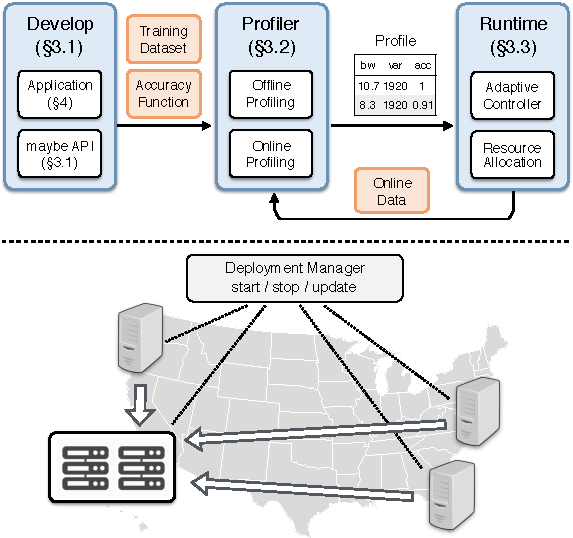
\includegraphics[width=.9\linewidth]{figures/system.pdf}
  \caption{\sysname{} Overview.}
  \label{fig:overview}
\end{figure}

\subsection{Structured Adaptation}
\label{sec:struct-adapt}

DAG: Applications are modelled as a directed acyclic graph (DAG) of
computation.  \texttt{maybe} operators to express the specification of
degradation. Our propose APIs do not require developers to be exact on the
quantity; integrating this into existing applications requires minimal effort.

We first consider a strawman solution: manual policies for
degradation. JetStream~\cite{rabkin2014aggregation} offers an example: ``if
bandwidth is insufficient, switch to sending images at 75\% fidelity, then 50\%
if there still isn't enough bandwidth. Beyond that point, reduce the frame rate,
but keep the images at 50\% fidelity.'' We identify the following issues with
this approach.

\para{Lack of precision:} These policies are often developer heuristics and
rarely backed up by measurements. First, there is no direct association of the
application accuracy with the 75\% fidelity configuration. Besides, their impact
on the data size is also not trivial.  While it seems intuitive that the level
of degradation will affect the data size, the precise impact is not always
straightforward. For example, one might think that reducing the frame rate by
50\% will half the data rate. When video encoding is employed, the inter-frame
difference will increased (P-frame size) when the frame rate is reduced. This
leads to a larger data size for each frame. \autoref{fig:h264} illustrates this
complex relationship with an example of H.264 encoding under four different
frame rates.

\para{Not scalable:} The strawman solution quickly leads to too many policies
when multiple degradation operations are involved or a fine-grained control is
desired. This manual process becomes tedious and error-prone. When too few rules
are provided, the application may oscillate between two rules: one that's too
aggressive (always faces insufficient bandwidth) and one that's too
conservative.

\para{Fixed:} Implemented as part of the application processing, it's fixed and
cannot be updated easily.

When using the above strawman solution, developers are forced to manually study
and measure the impact of individual degradation policy, prohibiting its wide
adoption in practice.

On the other extreme of the design spectrum, a completely developer-free
solution is not practical. While static analysis has been shown to optimize
application execution adaptively in a certain context~\cite{chun2011clonecloud},
they do not work well in our dataflow programming model. Static analysis is
prone to false positives: exploring wrong or unnecessary parameters. For
example, when the application is configured to generates statistics with a
\texttt{timed\_window} operation, static analysis may falsely detect the
duration parameter and alter the behavior of the application in an unexpected
way. Also, as we will illustrate in~\autoref{sec:profiling}, with each
introduced parameter, the profiling time increases drastically as all parameters
pose a combinatorial space.

Our system take a middle ground between these two extremes: developers use a
novel \texttt{maybe} API to annotate degradation operations without being exact
on the values. Think of these APIs as hints from developers: this operation,
when in use, will likely reduce the data size and affect the data fidelity;
however the exact impact is not clear.

The basic form of \texttt{maybe} operator takes two arguments: a knob and a
degradation function (see \autoref{tab:operators}). The knob indicates different
degradation levels; the function performs the actual degradation operation with
a configurable level. We restrict the type signature of the function that this
API can accept: $f(T, I) \Rightarrow I$. That is, the degradation function
should not alter the type of the stream. While this might seem a strong
restriction, when combined with \texttt{map} operator, the system is still
expressive enough. We describe our implementation and usage
in~\autoref{sec:implementation}.

Based on the \texttt{maybe} primitive, one can implement wrappers for common
degradation operations. For example, \texttt{maybe\_skip} will optionally
subsample a stream; and \texttt{maybe\_downsample} can adjust the image
resolution to a configured target. With this API, the example mentioned earlier
can now be implemented as follows:

\begin{lstlisting}
   let app = Camera::new((1920, 1080, 30))
      .maybe_downsample(vec![(1600, 900), (1280, 720)])
      .maybe_skip(vec![2, 5])
      .map(|frame| frame.show())
      .compose();
\end{lstlisting}

This snippet first instantiate a \texttt{Camera} source, which produces
\texttt{Stream<Image>} with 1920x1080 resolution and 30 FPS. Two degradation
operations are chained after the source: one that downsample the resolution to
either 1600x900 or 1280x720; the other skip the frame with a parameter of 2 or
5, resulting in 30/(2+1)=10 FPS or 30/(5+1)= 6 FPS. After the degradation,
images are shown on the display. In practice, further processing operators can
be chained.

While the API itself has simplified the specification of degradation, the exact
amount has to be known for precise rate adjustment at runtime. We then turn to
the second stage of our system that performs automatic profiling.

\begin{table*}
  \centering
  \begin{tabular}{ c r l }
    \toprule
    \multirow{7}{*}{Normal Operators}
    & \textit{map}(f: I $\Rightarrow$ O) & Stream<I> $\Rightarrow$ Stream<O> \\
    & \textit{filter}(f: I $\Rightarrow$ bool) & Stream<I> $\Rightarrow$
                                                 Stream<I> \\
    & \textit{skip}(i: Integer) & Stream<I> $\Rightarrow$ Stream<I> \\
    & \textit{sliding\_window}(count: Integer, f: Vec<I> $\Rightarrow$ O) & Stream<I> $\Rightarrow$
                                                                            Stream<O> \\
    & \textit{tumbling\_window}(count: Integer, f: Vec<I> $\Rightarrow$ O) & Stream<I> $\Rightarrow$
                                                                             Stream<O> \\
    & \textit{timed\_window}(time: Duration, f: Vec<I> $\Rightarrow$ O) & Stream<I> $\Rightarrow$
                                                                          Stream<O> \\
    & ... & ... \\
    \midrule
    \multirow{4}{*}{Degradation Operators}
    & \textit{maybe}(knobs: Vec<T>, f: (T, I) $\Rightarrow$ I) & Stream<I> $\Rightarrow$
                                                                 Stream<I> \\
    & \textit{maybe\_skip}(knobs: Vec<Integer>) & Stream<I> $\Rightarrow$ Stream<I> \\
    & \textit{maybe\_downsample}(knobs: Vec<(Integer, Interger)>) & Stream<Image> $\Rightarrow$ Stream<Image> \\
    & ... & ... \\
    \bottomrule
  \end{tabular}
  \caption{A comparison between normal stream processing operators and our
    degradation operators. \texttt{Vec<T>} represents a list of elements of type
    T. \texttt{Option<T>} indicates an optional element of type T which is
    either present \texttt{Some(T)} or absent \texttt{None}.}
  \label{tab:operators}
\end{table*}

\subsection{Automatic Profiling}
\label{sec:automatic-profiling}

The goal of our profiling stage is to explore the bandwidth-accuracy trade-off
and generate a \textit{profile} that is Pareto-optimal.

\subsubsection{Profiling Formalism}
\label{sec:formalize-profiling}

We first define terms and notations we will use. Each \texttt{maybe} operator
within an application corresponds to a knob $k$. Suppose the application has $n$
knobs, their combination forms a configuration $c = [k_{1}, k_{2},
... k_{n}]$. The set of all configurations $\mathbb{C}$ is the space that our
profiling system need to explore.

There are two mappings that we are particularly interested: a mapping from a
particular configuration to its bandwidth requirement $B(c)$ and the accuracy
measure $A(c)$. The Pareto-optimal set $\mathbb{P}$ can then be defined
(\autoref{eq:pareto}): for all $c \in \mathbb{P}$, there is no alternative
configuration $c'$ that requires less bandwidth while giving a higher accuracy.

{\small
\begin{equation}
  \mathbb{P} = \{ c \in \mathbb{C} : \{ c' \in \mathbb{C}: B(c') < B(c),
  A(c') > A(c) \} = \varnothing\}
  \label{eq:pareto}
\end{equation}
}%

\begin{table}
  \centering
  \begin{tabular}{r l}
    \toprule
    \textbf{Symbol} & \textbf{Description} \\
    \midrule
    $n$ & number of degradation operations \\
    $k_i$ & the \textit{i}-th degradation knob \\
    $c = [k_{1}, k_{2}, ... k_{n}]$ & one specific configuration \\
    $\mathbb{C}$ & the set of all configurations \\
    \midrule
    $B(c)$ & bandwidth requirement for $c$ \\
    $A(c)$ & accuracy measure for $c$ \\
    $\mathbb{P}$ & Pareto efficienct set \\
    \bottomrule
  \end{tabular}
  \caption{Notations used in profiling.}
  \label{tab:notations}
\end{table}

Since there is often no closed form relation for $B(c)$ and $A(c)$, our system
takes a data-driven approach: with a representative dataset and an
application-specific utility function, our system evaluates each configuration
for their bandwidth demand and accuracy degradation. The degradation could
either be measured against the groundtruth; or in the case when labelled dataset
is not available, the system uses the reference results when all degradations
are turned off.

\subsubsection{Offline Profiling}
\label{sec:offline-profiling}

Users provide a representative training data set. \para{Profiling is costly, ok
  for offline.}

\subsubsection{Online Profiling}
\label{sec:online-profiling}

When doing online profiling, we face two challenges: 1, lack of original data;
2, efficient profiling.

\para{Lack of groundtruth data or reference data.} During the online execution,
it's often not feasible to get groundtruth labelled data. Even with the
undegraded data may not be available.

\begin{itemize}[leftmargin=16pt]
\item Allocate some bandwidth for portions of undegraded data.
\item Use current best data as reference.
\end{itemize}

Although the first scheme seems to be incurring unnecessary bandwidth
consumption, when the runtime is probing for bandwidth, the data can enjoy a
free ride.

\para{Efficient profiling.} When doing profiling online, exhaustive exploring
all configurations is costly.

\begin{itemize}[leftmargin=16pt]
\item Parallel execution.
\item Smaller chunk of data.
\item Triggering profiling.
\end{itemize}

\subsection{Runtime Adaptation}
\label{sec:adaptation}

\begin{figure}
  \centering
  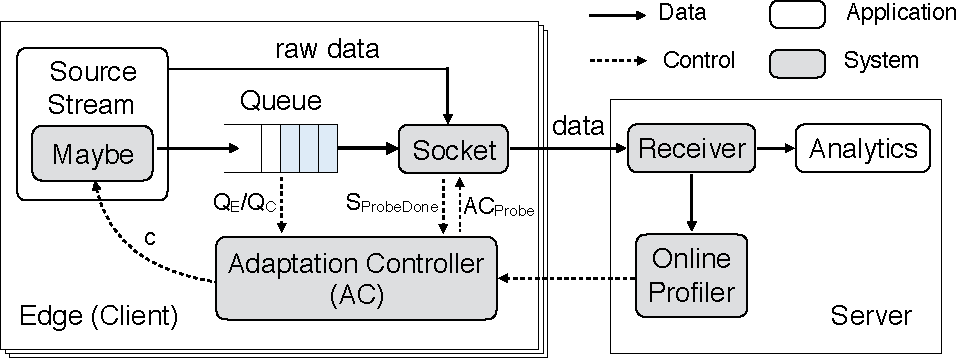
\includegraphics[width=\linewidth]{figures/runtime-adaptation.pdf}
  \caption{Runtime adaptation system architecture. The grey components are what
    \sysname{} provides.}
  \label{fig:runtime}
\end{figure}

At runtime, the user program is automatically converted to a client half and
server half; and \sysname{} abstracts the communication as well as rate
adaptation. \autoref{fig:runtime} shows our runtime architecture.

\para{Object-level queue:} The queue bridges data generation and
the network capacity. It transmits data as fast as the network can handle and
detects congestion when the queue grows.

\para{Congestion controller:} Our first prototype used the queue length as a
signal for congestions, this turns out to be a bad match as the degradation
operation may change object arrival rate (e.g.\,lower frame rate for video). Our
next version uses data size, but it also leads to long latency when the
degradation changes individual object size (e.g.\,lower resolution). Our current
design uses an adaptive size: given current configuration and the profile, the
queue learns the desired data generation rate (bps), and with a user configured
latency, the queue derive the congestion watermark.

\resizebox{!}{!}{
  \begin{tikzpicture}[
  state/.style = { draw, very thick, fill=white, rounded corners=1em,
    minimum height=3em, minimum width=7em, node distance=7em, font={\bfseries},
    align=center },
  edge portion/.style = { black, thick },
  transition/.style = { edge portion, -> },
  algorithm/.style = { draw, thin, fill=white },
  ]

  \node [state] (startup) {
    STARTUP };
  \node [state] (congestion) [right=of startup] {CONGESTION};
  \draw [transition] (startup) -- (congestion)
  node [midway, auto] {Q.Congestion};

  \node [state] (steady) [below=of congestion] {STEADY};

  \draw [transition] ($(congestion.south west)!0.4!(congestion.south east)$)
  to node[midway, sloped, below] {Q.NoQueue}
  ($(steady.north west)!0.4!(steady.north east)$);

  \draw [transition] ($(steady.north west)!0.6!(steady.north east)$)
  to node[midway, sloped, below] {Q.Congestion}
  ($(congestion.south west)!0.6!(congestion.south east)$);

  \node [state] (probe) [left=of steady] {PROBE};

  \draw [transition] ($(steady.south west)!0.6!(steady.north west)$)
  -- ($(probe.south east)!0.6!(probe.north east)$)
  node[midway, auto, swap] {Q.Probe};

  \draw [transition, <-] ($(steady.south west)!0.4!(steady.north west)$)
  -- ($(probe.south east)!0.4!(probe.north east)$)
  node[midway, auto, align=left] {Q.Congestion | \\ IO.ProbeDone};

\end{tikzpicture}


%%% Local Variables:
%%% mode: latex
%%% TeX-master: "sosp17"
%%% End:

}

\para{Bandwidth Measurement:} The receiver delivers the received data to
application. In the meantime, it measures the effective throughput between each
client-server pair as an indication of current bandwidth. To avoid spikes in the
bandwidth measurement, exponential smoothing is employed. While the receiver
performs bandwidth measurement every second, it does not send the information
back to each client.  avoid unnecessary communication, the client requests the
measurement only when congestion is detected.

\para{Policy Manager:} Upon receiving signals from congestion controller, it
performs an RPC request to the server for current bandwidth measurement. With
the learned profile, it determines the degradation level and start the actual
degradation strategy. The bandwidth specification in the learned profile is the
required bandwidth, the policy manager usually takes a conservative approach:
using a constant rate ALPHA to adjust the available bandwidth. When the
congestion is resolved, the policy manager gradually reduce the degradation
level (additive increase phase).

\para{Degrade:} The actual degradation operation is rather simple. Operators
based on the \texttt{maybe} API supports a \texttt{set} function that would
change the internals of the operator. The \texttt{set} function is invoked when
degradation is needed.

We then outline the rate-based congestion control algorithm.

\todo{One figure about states and state transitions during the congestion
  control}.

%%% Local Variables:
%%% mode: latex
%%% TeX-master: "sosp17"
%%% End:

\section{Implementation}
\label{sec:implementation}

While our proposed API is general and not language specific, we have implemented
\sysname{} prototype in Rust (\textasciitilde 4000 lines of code). \sysname{} is
open source on GitHub.\footnote{URL elided for anonymity.}  Applications use
\sysname{} as a library and configure the execution mode---profiling, runtime as
client, or runtime as server---with command line arguments.

% \begin{figure}
%   \centering
%   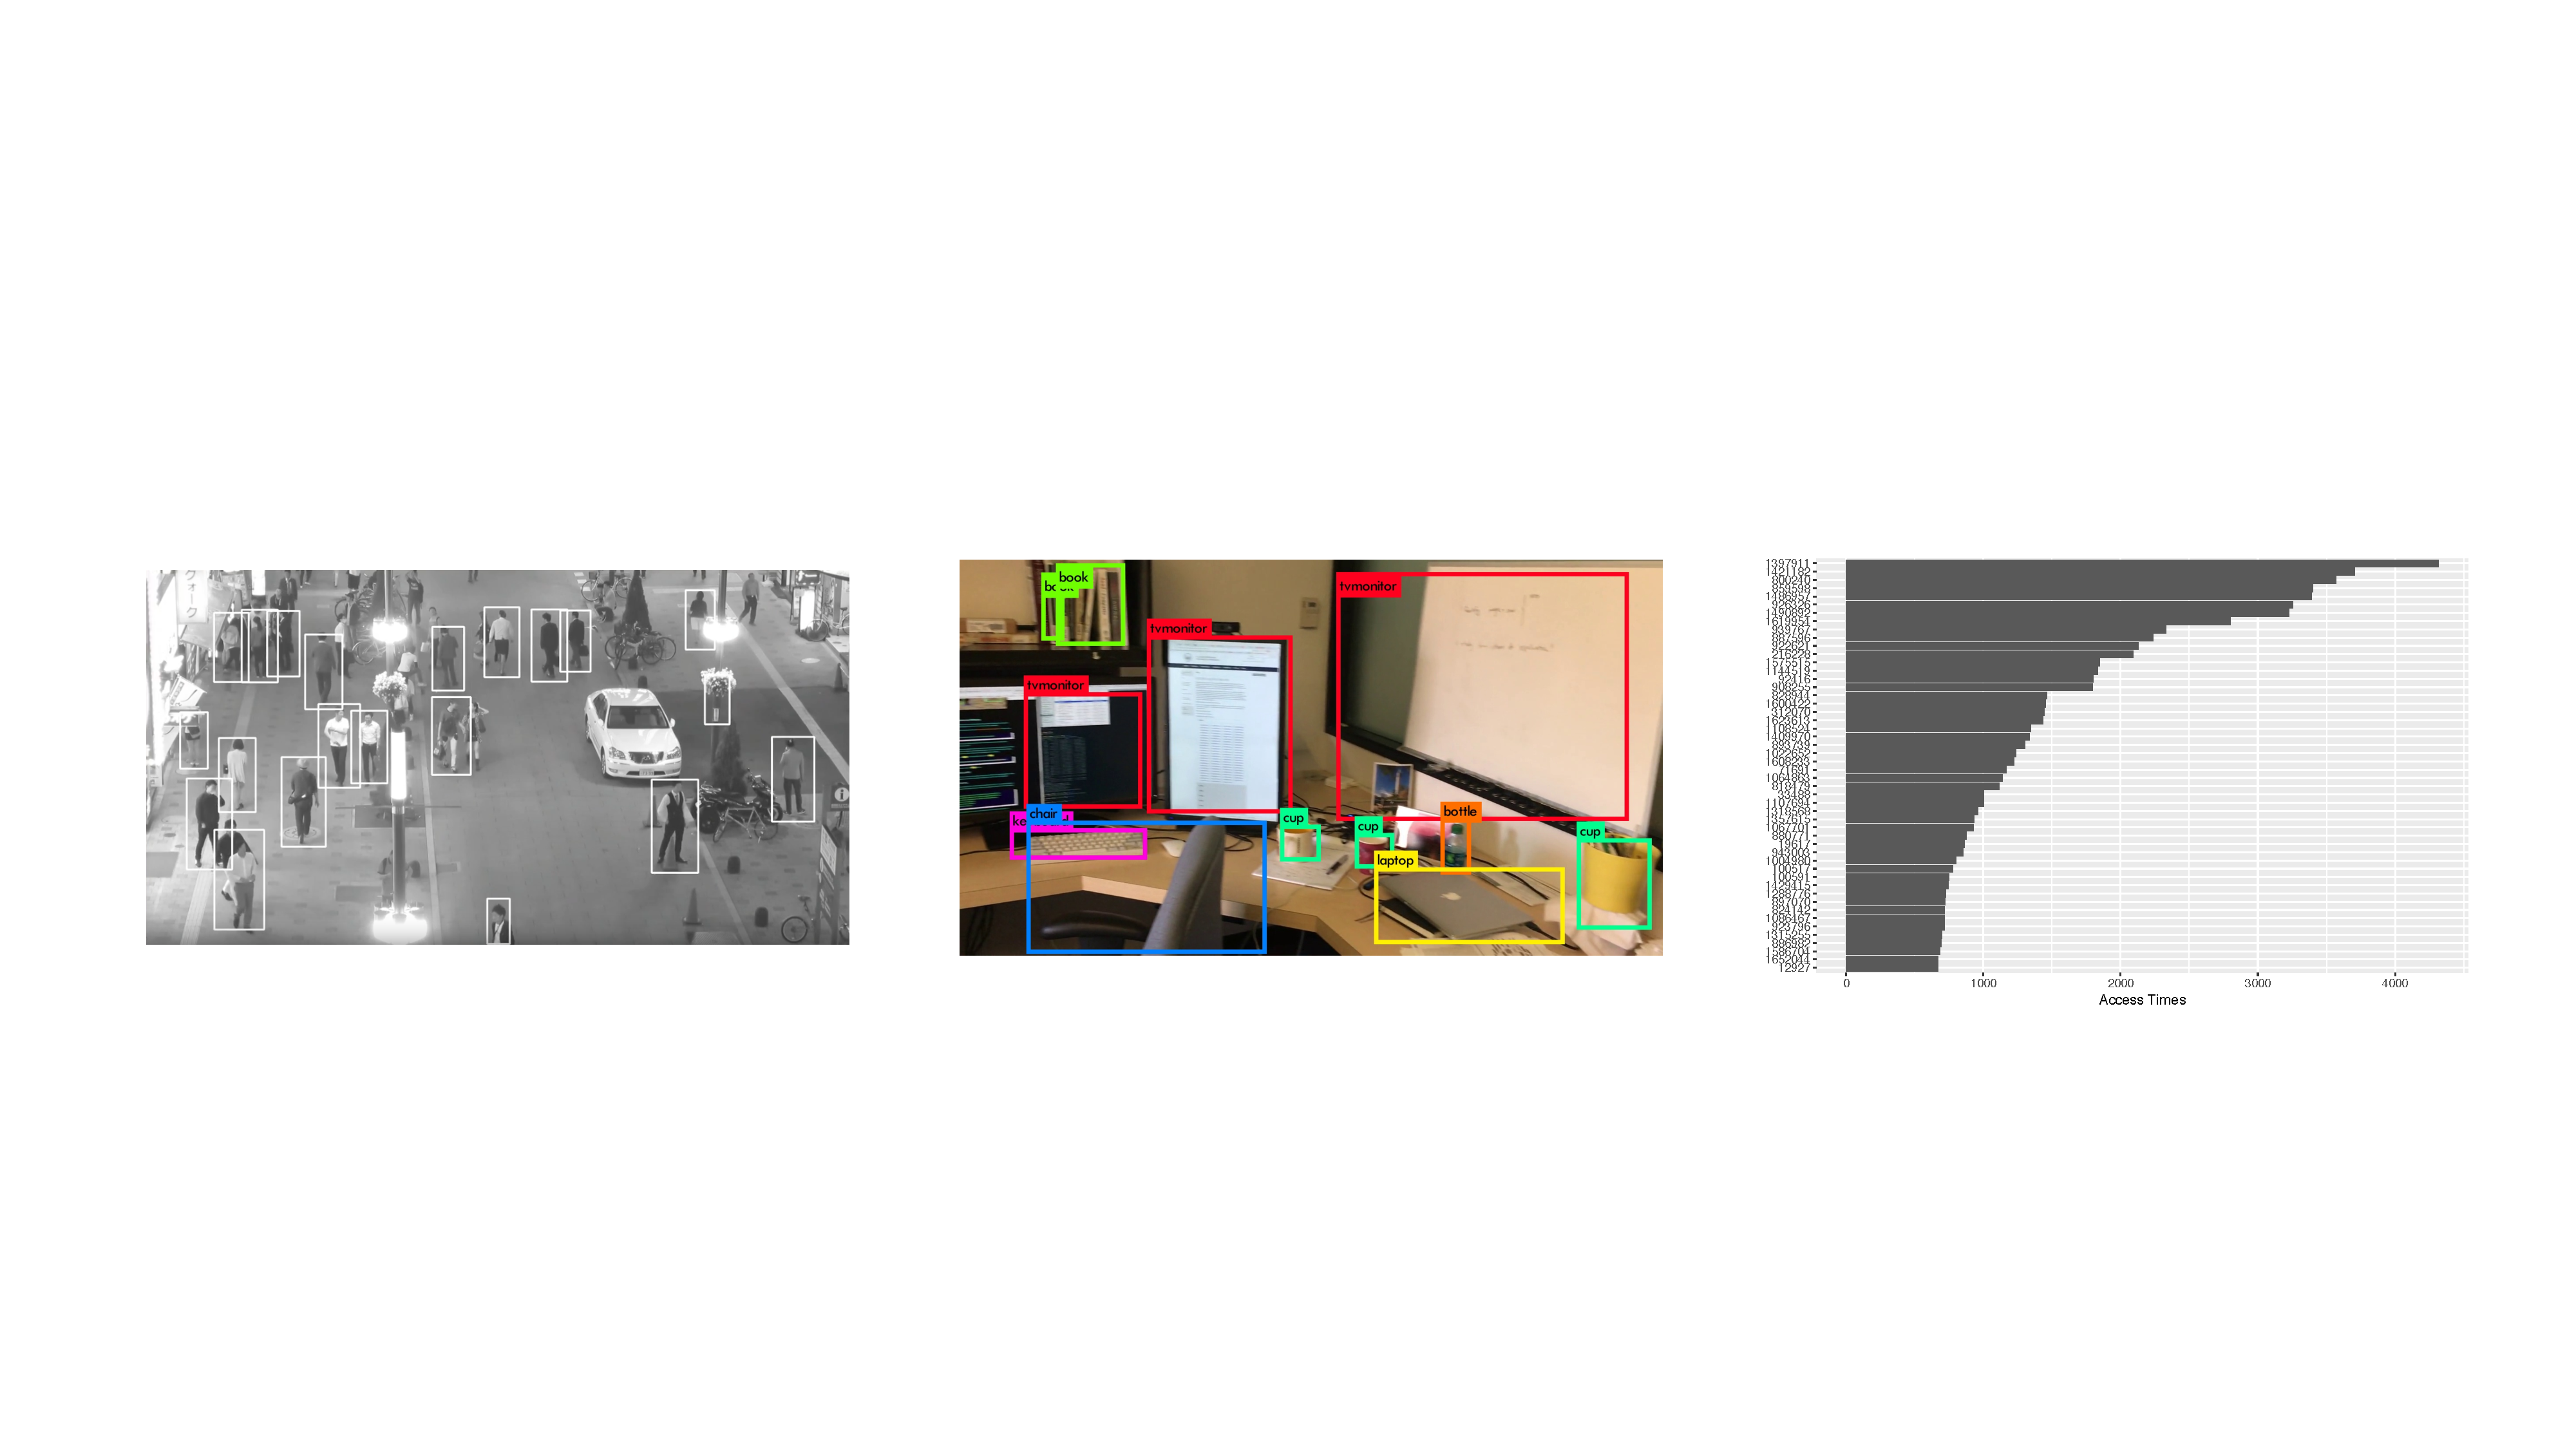
\includegraphics[width=\columnwidth]{figures/apps.pdf}
%   \caption{Three \sysname{} applications: augmented reality, pedestrian
%     detection, and distributed Top-K.}
%   \label{fig:three-apps}
% \end{figure}

\begin{table}
  \footnotesize
  \centering
  \begin{tabular}{c c c c}
    \toprule
    Application & Knobs & Accuracy & Dataset \\
    \midrule
    \specialcell{Augmented\\Reality}
                & \specialcell{resolution \\ frame rate \\ quantization }
                & F1 score~\cite{Rijsbergen:1979:IR:539927}
                & \specialcell{iPhone video clips\\training: office (24
    s)\\testing: home (246 s)} \\
    \midrule
    \specialcell{Pedestrian\\Detection}
                & \specialcell{resolution \\ frame rate \\ quantization }
                & F1 score
                & \specialcell{MOT16~\cite{milan2016mot16}\\training: MOT16-04\\testing: MOT16-03} \\
    \midrule
    \specialcell{Log Analysis\\(Top-K, K=50)}
                & \specialcell{head (N) \\ threshold (T) }
                & \specialcell{Kendall's $\tau$~\cite{abdi2007kendall}}
                & \specialcell{\href{https://www.sec.gov}{SEC.gov} logs~\cite{edgarlog} \\ training: 4 days \\
    testing: 16 days} \\
    \bottomrule
  \end{tabular}
  \vspace{0.5em}
  \caption{Application details.}
  \label{tab:apps}
  \vspace{-1em}
\end{table}

Using \sysname{}, we have built three applications: augmented reality (AR) that
recognizes nearby objects on mobile phones, pedestrian detection (PD) for
surveillance cameras, and a distributed log analysis to extract the Top-K mostly
accessed files (TK). \autoref{tab:apps} summarizes the application-specific
parts: knobs, accuracy functions, and datasets.

\para{Augmented Reality.} We target at augmented reality applications running on
mobile phones that recognize nearby objects by offloading the heavy computation
elsewhere, e.g.\,the cloud. Our implementation uses OpenCV
3.1~\cite{opencvlibrary} for image-related operations and YOLO~\cite{darknet13,
  redmon2016yolo9000}, a GPU-enabled pre-trained neural network, for object
recognition. Videos are encoded with H.264~\cite{richardson2011h}. Our
implementation uses GStreamer~\cite{gstreamer} with \texttt{x264enc} plugin
(\texttt{zerolatency} and constant quality). The quantization factor affecting
encoding quality becomes a knob in addition to image resolutions and frame
rates.

Object recognition returns a list of bounding boxes with the type of the
object. Each bounding box is a rectangle with normalized coordinates on the
image. We compare the detection against the reference result from raw data, and
declare it success if the intersection over union (IOU) is greater than
50\%~\cite{everingham2010pascal} and the object type matches. We use F1
score~\cite{Rijsbergen:1979:IR:539927} as the accuracy function. In terms of
dataset, we collected our own video clips: the training data is a 24-second long
video of an office environment; the test data is a 246-second long video of a
home environment.

\para{Pedestrian Detection.} This application analyzes streams of videos from
installed CCTV cameras and detects pedestrians inside. We use a similar setup
(OpenCV and GStreamer) as our augmented reality application except for the
analytical function. To detect pedestrians, we use GPU-accelerated histogram of
oriented gradients (HOG)~\cite{dalal2005histograms} with the default linear SVM
classifier from OpenCV. Because we do not recognize individual pedestrians, a
successful detection in this case only requires matching the bounding box. Our
evaluation uses MOT16 dataset~\cite{milan2016mot16} for both profiling and
runtime.

\begin{figure}
  \centering
  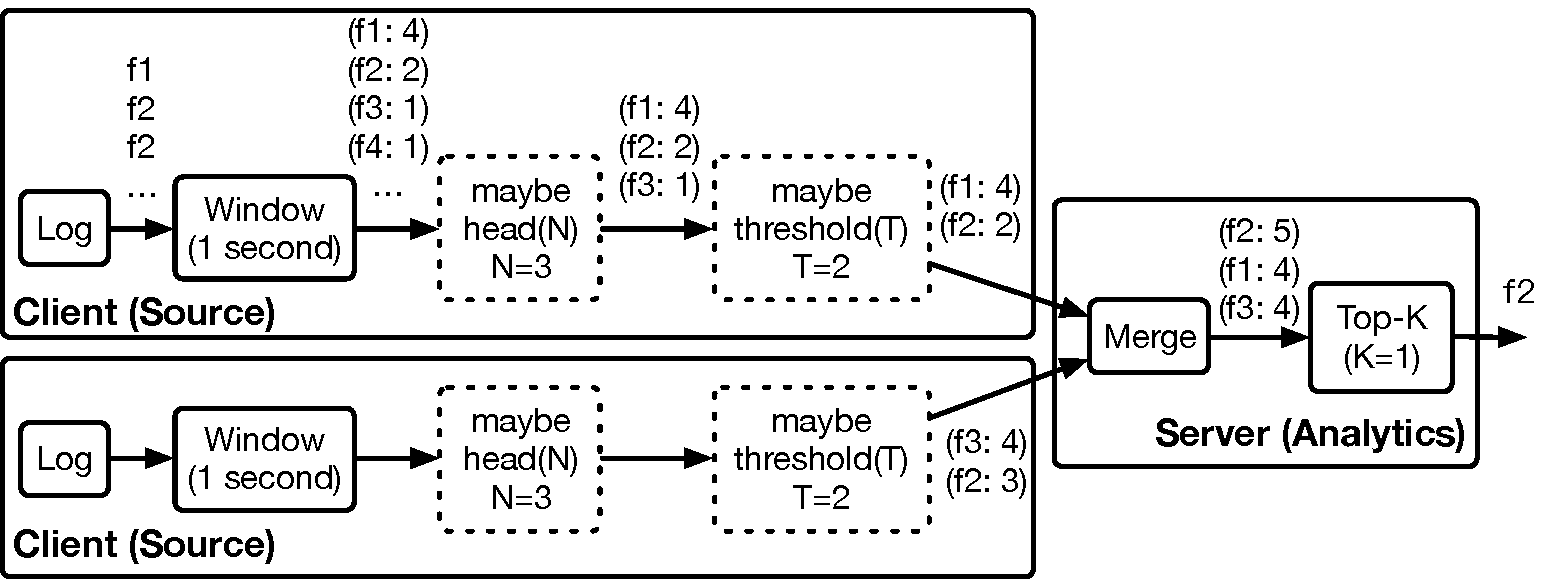
\includegraphics[width=\columnwidth]{figures/topk.pdf}
  \caption{A distributed Top-K application with two degradation operations:
    \texttt{head} and \texttt{threshold}. In this example, \texttt{f2}, which is
    not in Top-1 for either client, becomes the global Top-1 after the merge. It
    would have been purged if the clients use threshold T=3, demonstrating
    degradation that reduces data sizes affects fidelity.}
  \label{fig:topk}
  \vspace{-0.5em}
\end{figure}

\para{Distributed Top-K.} This application aggregates machine logs from
geo-distributed servers to find out the Top-K most accessed files, similar to
many Top-K queries~\cite{babcock2003distributed}. \autoref{fig:topk} illustrates
our processing pipeline with two degradation operations. First each source node
summarizes the log using \texttt{Window} operator to reduce the data size, a
pre-processing step. As many real-world access patterns follow a long tail
distribution, there is a large-but-irrelevant tail that contributes little to
the final Top-K. Each source node then filters the tail: (1) head(\texttt{N})
takes the top \texttt{N} entries; (2) threshold(\texttt{T}) filters small
entries whose count is smaller than \texttt{T}. These two operations affect the
final result and the exact impact depends on data distribution. We implement
these two operators by using \sysname{}'s \maybe{} abstraction.

To measure the accuracy, we need to compare the correlation between two ranked
list. Kendall's~$\tau$~\cite{abdi2007kendall} is a correlation measure of the
concordance between two ranked list. The output ranges from \(-1\) to 1,
representing no agreement to complete agreement. To integrate with \sysname{},
we convert Kendall's~$\tau$ to [0, 1] with a linear transformation. For our
evaluation, we set K as 50 and use Apache log files that record and store user
access statistics for the \href{https://www.sec.gov}{SEC.gov} website. The logs
are split into four groups, simulating four geo-distributed nodes monitoring web
accesses. To match the load of popular web servers, we compress one hour's logs
into one second.

%%% Local Variables:
%%% mode: latex
%%% TeX-master: "../awstream"
%%% End:

\section{Evaluation}
\label{sec:evaluation}

The evaluation consists of four parts:

\begin{itemize}
\item Application profiles (\autoref{fig:all-profiles})
\item Online Profiling (\autoref{fig:online-profiling-comparison},
  \autoref{fig:parallel}, \autoref{fig:trigger})
\item Runtime Adaptation (\autoref{fig:all-runtime})
\item Multi-task Scheduling (\autoref{fig:multitask})
\end{itemize}

\subsection{Application Profiles}
\label{sec:application-profiles}

Our system learned the application profiles for all three applications (shown in
\autoref{fig:all-profiles}). From these profiles, we make the following three
observations:

\para{Optimal strategy is achieved with multiple dimensions.} In each profile,
in addition to the Pareto-optimal strategies, we show the performance if only
one dimension is tuned. As show in the figure, they almost always lead to a
sub-optimal performance.

\para{Different dimensions have different impact for the same application.}
For pedestrian detection, tuning resolution leads to a quicker degradation in
comparison to tuning frame rate.

\para{The same dimension has different impact for different applications.}
If we compare two video analytics applications, pedestrian detection and
augmented reality, we see how tuning each dimension affects the performance
differently.

\begin{figure*}
  \centering
  \begin{subfigure}[t]{0.33\textwidth}
    \centering
    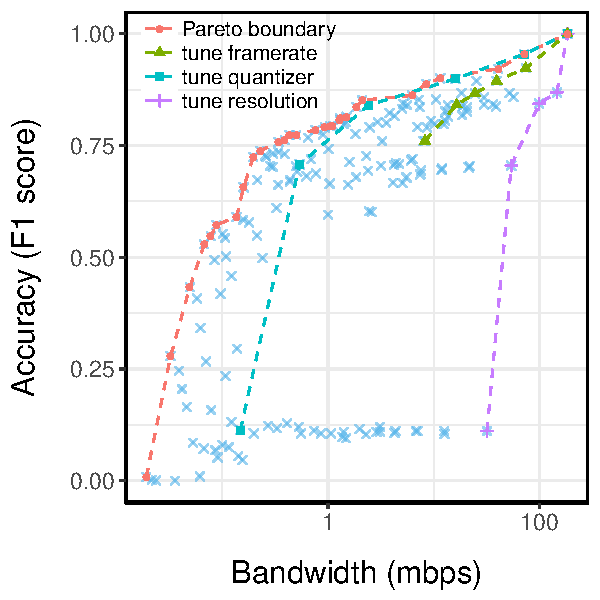
\includegraphics[width=\textwidth]{figures/ped-profile.pdf}
    \caption{Pedestrian Detection}
    \label{fig:pd-profile}
  \end{subfigure}
  ~
  \begin{subfigure}[t]{0.33\textwidth}
    \centering
    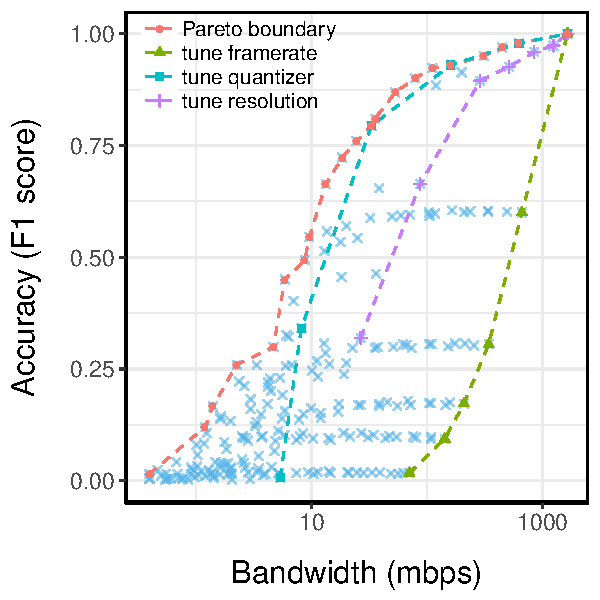
\includegraphics[width=\textwidth]{figures/darknet-profile.pdf}
    \caption{Augmented Reality}
    \label{fig:ar-profile}
  \end{subfigure}
  ~
  \begin{subfigure}[t]{0.33\textwidth}
    \centering
    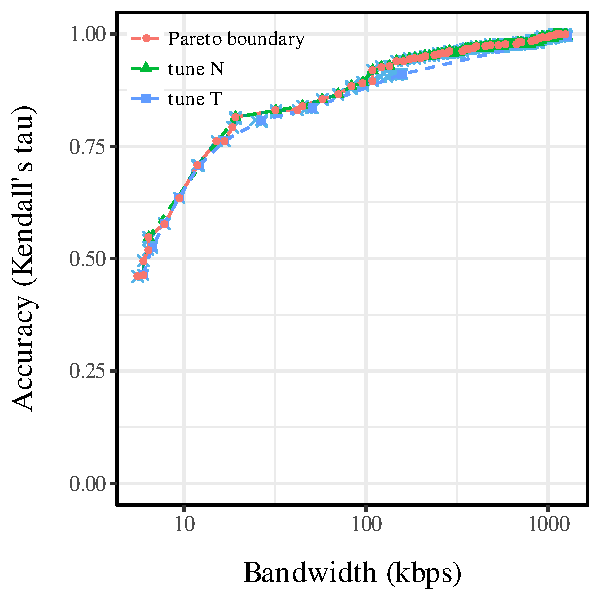
\includegraphics[width=\textwidth]{figures/topk-profile.pdf}
    \caption{Top-k}
    \label{fig:tk-profile}
  \end{subfigure}
  \caption{Application profiles.}
  \label{fig:all-profiles}
\end{figure*}

\subsection{Efficient Online Profiling}
\label{sec:online-profiling}

First, we validate the necessity for online profiling. We compare two adaptation
scheme: one with the offline learned profile; the other enabled with online
profiling. \autoref{fig:online-profiling-comparison} shows the performance
difference. Initially, both schemes work similarly. Overtime, when the data
distribution changes, the offline-learned profile doesn't match with the newly
generated data, leading to accuracy deterioration. System enabled with online
profiling is able to track the data and offers high accuracy.

\begin{figure}
  \centering
  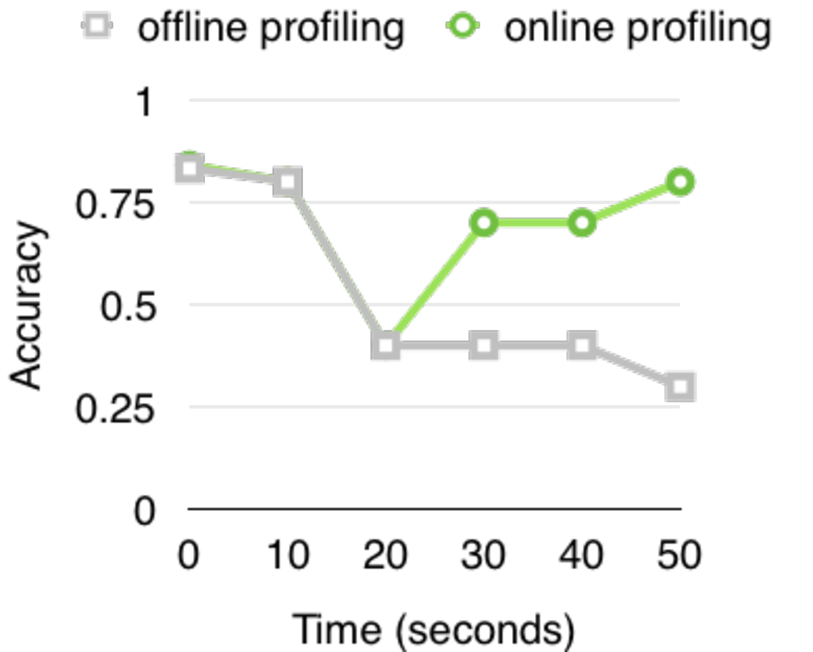
\includegraphics[width=\columnwidth]{figures/offline-online-profiling.pdf}
  \caption{The case for online profiling}
  \label{fig:online-profiling-comparison}
\end{figure}

While online profiling is beneficial, doing it naively faces the combinatorial
space search. This is different from the offline profiling that doesn't have
much time or resource constrain.

We evaluate our proposed solutions regarding the efficiency.

\para{Degradation-aware parallel profiling:} In the offline learned profile, we
have the measured time required to run for each configuration. Our parallel
profiling takes the measurements as input and generates a parallel profiling
schedule: Compare strategies for profiling.  \autoref{fig:parallel} shows our
profiling scheduling in comparison with a naive scheduler.

\begin{figure}
  \centering
  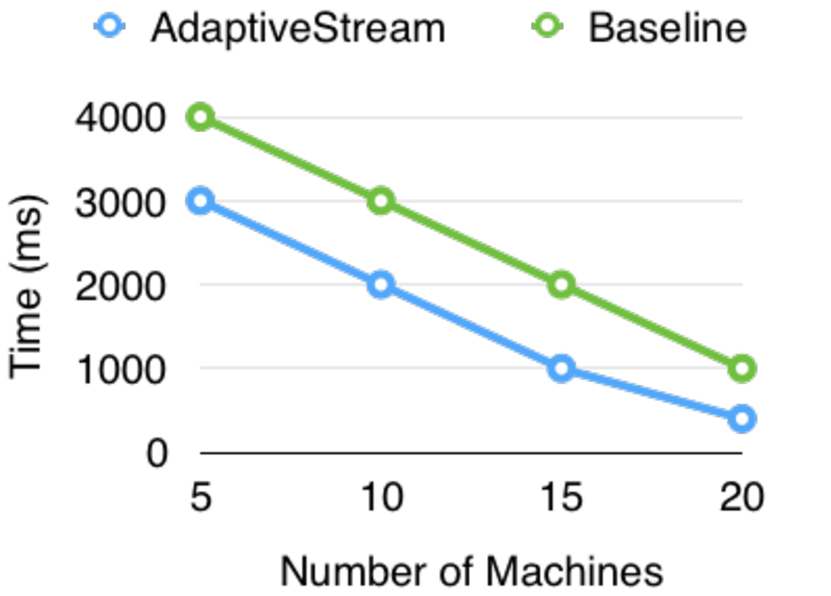
\includegraphics[width=\columnwidth]{figures/parallel-placeholder.pdf}
  \caption{Degradation-aware parallel scheduling}
  \label{fig:parallel}
\end{figure}

\para{Trigger-based profiling:} Only start the profiling when there is
substantial difference. \autoref{fig:trigger} shows the savings in trigger-based
profiling.

\begin{figure}
  \centering
  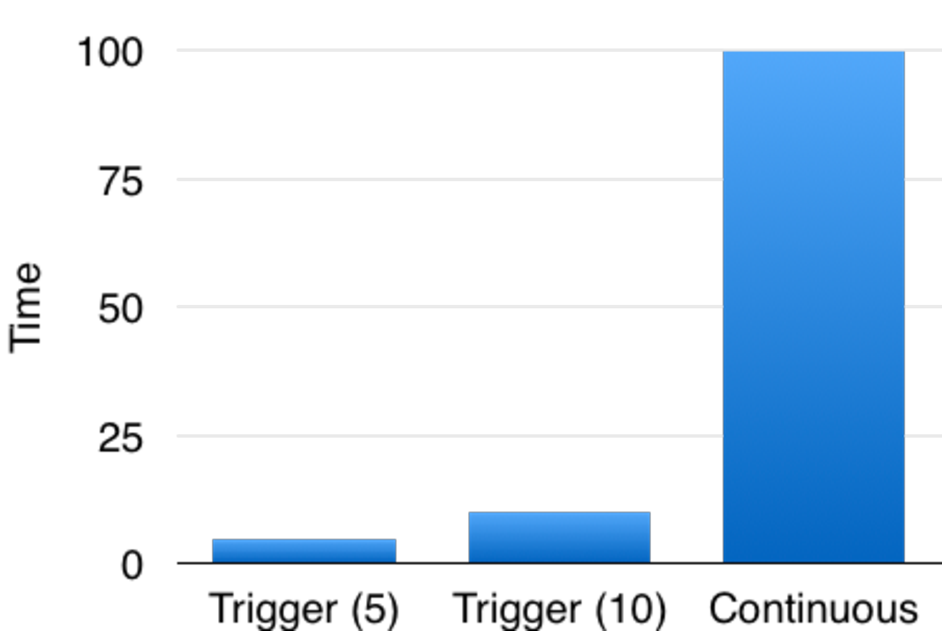
\includegraphics[width=\columnwidth]{figures/trigger.pdf}
  \caption{Trigger-based profiling}
  \label{fig:trigger}
\end{figure}

\subsection{Runtime Adaptation}
\label{sec:runtime-adaptation}

\begin{figure*}
  \centering
  \begin{subfigure}[t]{0.33\textwidth}
    \centering
    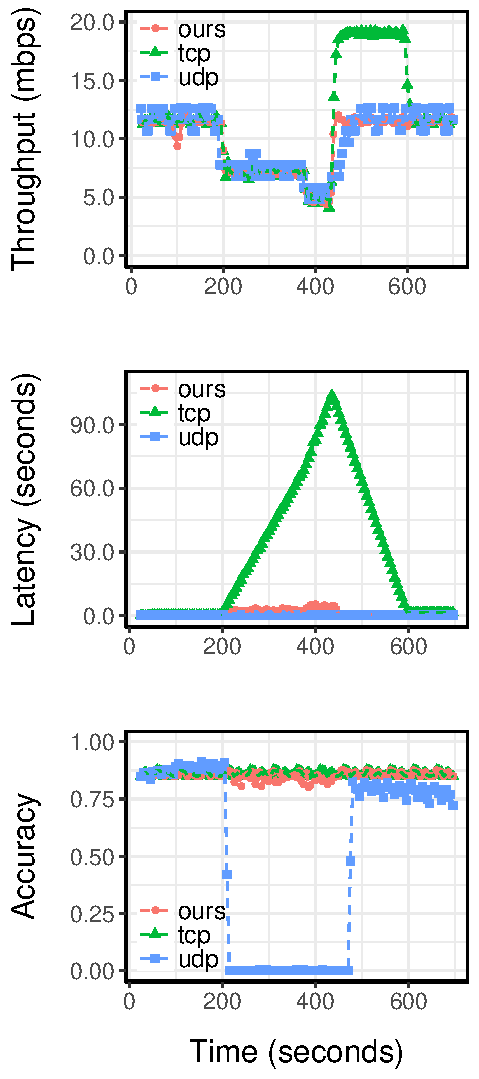
\includegraphics[width=\textwidth]{figures/ped-runtime-verticle.pdf}
    \caption{Pedestrian Detection}
    \label{fig:pd-runtime}
  \end{subfigure}
  ~
  \begin{subfigure}[t]{0.33\textwidth}
    \centering
    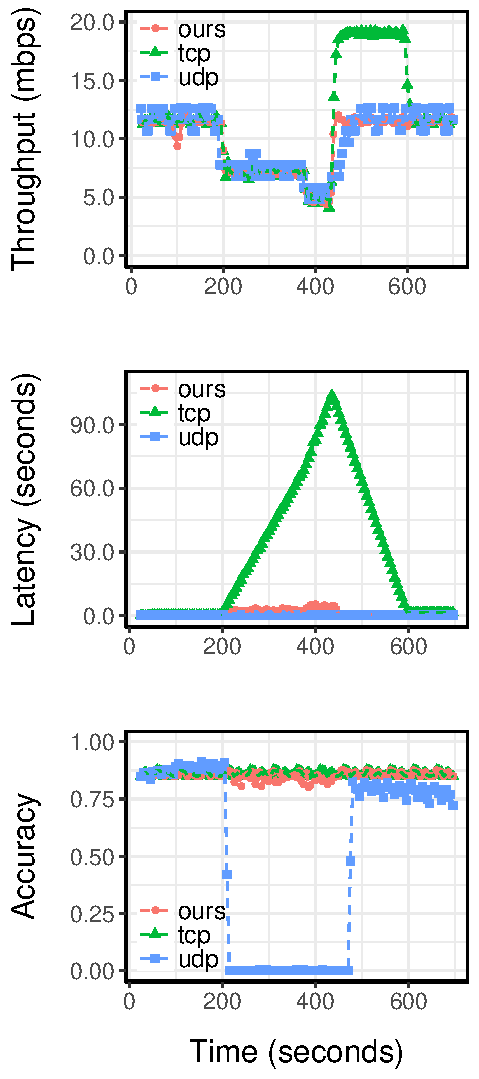
\includegraphics[width=\textwidth]{figures/ped-runtime-verticle.pdf}
    \caption{Augmented Reality}
    \label{fig:ar-runtime}
  \end{subfigure}
  ~
  \begin{subfigure}[t]{0.33\textwidth}
    \centering
    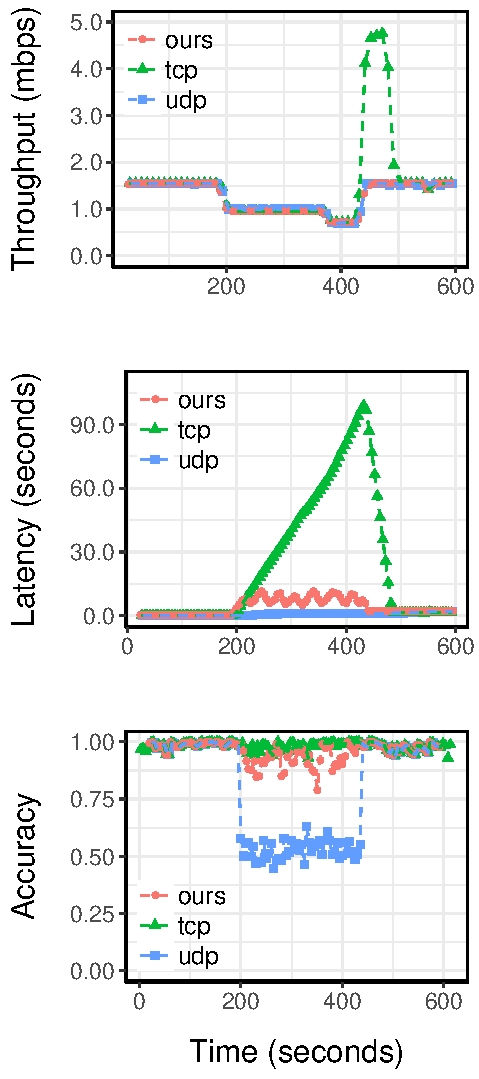
\includegraphics[width=\textwidth]{figures/topk-runtime-verticle.pdf}
    \caption{Top-k}
    \label{fig:tk-runtime}
  \end{subfigure}
  \caption{Application profiles.}
  \label{fig:all-runtime}
\end{figure*}

\subsection{Multi-task Scheduling}
\label{sec:multi-task-sched}

\begin{figure}
  \centering
  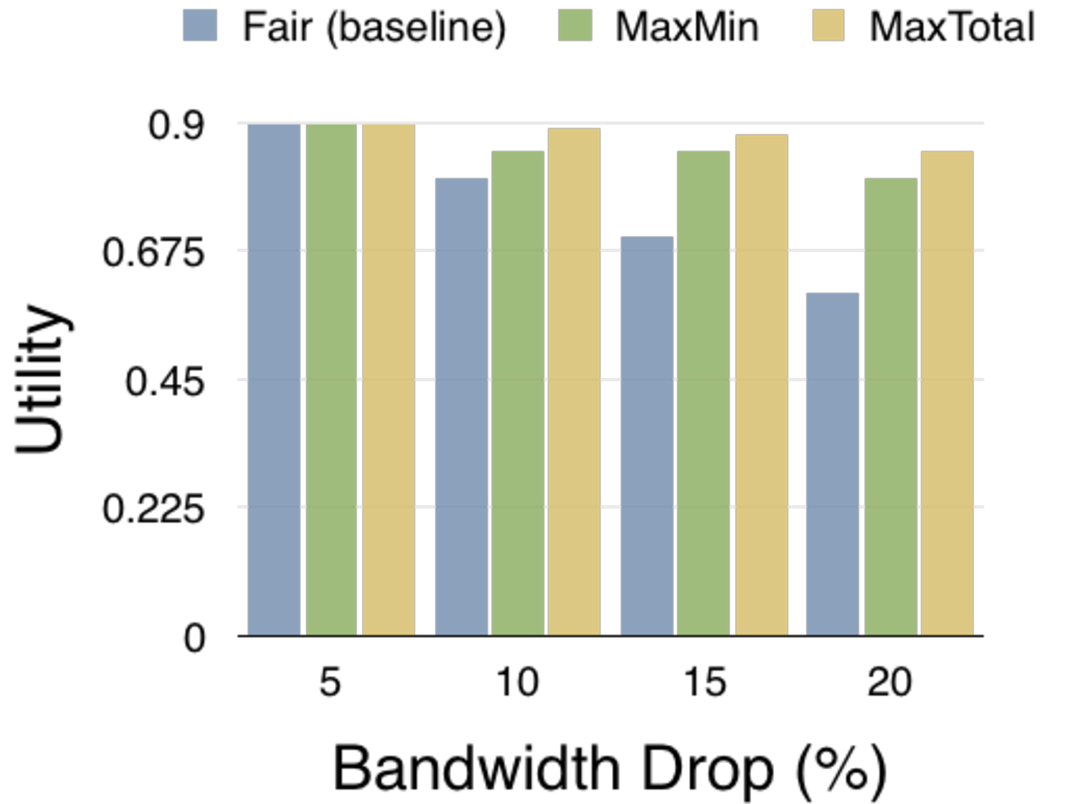
\includegraphics[width=\columnwidth]{figures/multitask.pdf}
  \caption{Multitask Scheduling}
  \label{fig:multitask}
\end{figure}

%%% Local Variables:
%%% mode: latex
%%% TeX-master: "sosp17"
%%% End:

\section{Related Work}
\label{sec:related-work}

The work most closely related to \sysname{} is
JetStream~\cite{rabkin2014aggregation}. Both systems target at wide-area
streaming analytics. JetStream proposes to use aggregation and \textit{manual}
degradation policies to achieve responsiveness in the presence of bandwidth
fluctuation. We've discussed its limitations in \autoref{sec:motivation}.

We divide other related works into stream processing systems, approximate
analytics, WAN-aware systems and adaptive video streaming.

\paraf{Stream processing systems:} Streaming databases, such as
Borealis~\cite{abadi2005design},
TelegraphCQ~\cite{chandrasekaran2003telegraphcq}, are the early academic
explorations. They pioneered the usage of dataflow models with specialized
operators for stream processing. Recent research projects and open-source
systems, such as MillWheel~\cite{akidau2013millwheel},
Storm~\cite{toshniwal2014storm}, Heron~\cite{sanjeev2015twitter}, Spark
Streaming~\cite{zaharia2013discretized}, Apache Flink~\cite{carbone2015apache},
primary focus on fault-tolerant streaming in the context of a single
cluster. While our work has a large debt to the prior streaming work, \sysname{}
is designed for the wide area and explicitly trades data fidelity for data
freshness. In contrast, these stream processing systems often choose to throttle
the source when backpressure happens.

\para{Approximate analytics:} The idea of degrading computation fidelity for
responsiveness has also been explored in other contexts. For SQL queries, online
aggregation~\cite{hellerstein1997online}, BlinkDB~\cite{agarwal2013blinkdb} and
GRASS~\cite{ananthanarayanan2014grass} speed up queries with partial data based
on a statistical model of SQL operators. For real-time processing,
MEANTIME~\cite{farrell2016meantime} uses approximation to guarantee satisfying
real-time deadlines. For video processing, VideoStorm~\cite{zhang2017live}
optimizes video stream \textit{processing} within lager clusters with
approximation and delay-tolerance for resource management and allocation. The
trade-off between available resource and application accuracy is a common theme
among all these works. \sysname{} targets at wide-area streaming analytics, an
emerging application domain especially with the advent of IoT.

\para{WAN-aware systems:} The main challenge in designing geo-distributed
systems is to cope with high latency and limited bandwidth. While some research
projects, such as Vivace~\cite{cho2012surviving}, assume the network can
prioritize a small amount of critical data to avoid delays even under
congestion, most systems reduce data transfer in the first place to avoid
congestion. For example, LBFS~\cite{muthitacharoen2001low} exploits similarities
between files or versions of the same file. Over the past few years, we have
seen a plethora of geo-distributed analytical frameworks:
WANalytics~\cite{vulimiri2015wananlytics}, Geode~\cite{vulimiri2015global},
Iridium~\cite{pu2015low}, Pixida~\cite{kloudas2015pixida},
Clarinet~\cite{viswanathan2016clarinet}, etc. They minimize data movement by
incorporating heterogeneous wide-area bandwidth information into query
optimization and data/task placement. While effective in improving analytics
efficiency, they focus on batch analytics such as MapReduce tasks or SQL
query. Such tasks are often executed once, with little real time constrain. In
contrast, \sysname{} focuses on streaming analytics that process streams of data
continuously in real time.

%% - Pixida~\cite{kloudas2015pixida} minimizes data movement across inter-DC
%% links by solving a traffic minimization problem in data analytics.

%% - Iridium~\cite{pu2015low} optimizes data and task placement jointly to
%% achieve an overall low latency goal.

%% - Clarinet~\cite{viswanathan2016clarinet} incorporate bandwidth information
%% into query optimizer to reduce data transfer.

%% WheelFS~\cite{stribling2009flexible}

%% Geode~\cite{vulimiri2015global} develops input data movement and join
%% algorithm selection strategies to minimize WAN bandwidth usage.

%% WANalytics~\cite{vulimiri2015wananlytics} focuses on batch analytics.

%% SWAG~\cite{hung2015scheduling} coordinates compute task scheduling across
%% DCs.

%% \cite{heintz2015towards} discusses the complex tradeoffs involved in
%% wide-area analytics.

\para{Adaptive video streaming:} Designing a good adaptation strategy to improve
QoE for video streaming has been a hot topic. Research
projects~\cite{yin2015control, sun2016cs2p} and industrial efforts
HLS~\cite{pantos2016http}, DASH~\cite{sodagar2011mpeg,
  michalos2012dynamic}. Despite fruitful, their results are not directly
transferable to the wide-area streaming analytics. \sysname{} attempts at a
generalization with \maybe{} APIs to allows more custom control over what
parameters can be adjusted. \sysname{} is not competing with video streaming
technologies. Instead, our APIs are extensible to incorporate techniques such as
video encoding (H.264~\cite{richardson2011h} or VP9~\cite{grange2016vp9}). The
main contribution of \sysname{} here is to provide a system for arbitrary
streaming analytics to benefit from adaptation.

%% TCP, for example, adapts to available bandwidth by controlling the congestion
%% window with AIMD~\cite{jacobson1988congestion}.  Previous work has proposed
%% modifications to TCP for specific contexts. For streaming over TCP, Goel et
%% al.~\cite{goel2008low} proposes adaptive buffer-size tuning. For the cloud,
%% Adaptive TCP~\cite{wu2013adaptive} proposes to modify the congestion control
%% behavior based on flow size for the cloud.

% \para{Scheduling and allocation:} Resource allocations in the cloud is how to
% efficiently allocate tasks.  In the wide area, we face fundamental limit that
% therefore degradation is more effective. For multiple tasks, Existing
% allocations are for resources without considering application trade-offs.
% MediaNet~\cite{hicks2003user} uses both local and online global resource
% scheduling to improve user performance and network utilization, and adapts
% without requiring underlying support for resource
% reservations. VideoStorm~\cite{zhang2017live} primarily focuses on cluster
% resource allocation among video queries. For wide-area, the resource
% allocation is limited. We do not control the capacity; but still we can
% allocate the available bandwidth.

% Performance modeling: CherryPick~\cite{alipourfard2017cherrypick},
% Ernest~\cite{venkataraman2016ernest}.
%% Dolly~\cite{ananthanarayanan2013effective}.
%% \para{Program Synthesis:}

%%% Local Variables:
%%% mode: latex
%%% TeX-master: "sosp17"
%%% End:

\section{Conclusion}
\label{sec:conclusion}

We have proposed \sysname{}, an adaptive stream processing system for wide-area
streaming analytics. Developers express data degradation operations with
\maybe{} APIs, and our system performs automatic offline and online profiling to
learn a Pareto-optimal adaptation strategy. \sysname{} runtime executes
applications with network-condition awareness. By adapting the data rate to
available bandwidth, we achieve low latency (sub-second) and high accuracy
simultaneously. The profiles are also useful to control and allocate bandwidth
among competing applications.

In summary, \sysname{} allows resilient execution of wide-area streaming
analytics over time and continuously with minimal developer effort.

%%% Local Variables:
%%% mode: latex
%%% TeX-master: "sosp17"
%%% End:


\bibliographystyle{ACM-Reference-Format}
\bibliography{sosp17}

\end{document}

%%% Local Variables:
%%% mode: latex
%%% TeX-master: t
%%% End:
